\chapter{Third-Party Code and Libraries}

\section{Images}
The unit iconography was taken from http://game-icons.net which is a resource of thousands of free, customizable icons. All icons are provided under the terms of the Creative Commons 3.0 license.

Unit themselves images were borrowed from a sprite sheet found at\\ http://i54.photobucket.com/albums/g85/FeatherofDeath/ImperialSheet-2.png. No license was found accompanied with this sprite sheet so these images are used solely for testing and would not be released with the final product.

Other icons were from http://icomoon.io which creates custom icon fonts but also allows for icons to be exported as image files. Icons used are provided under the terms of the Creative Commons 3.0 license.

\section{osmdroid}
Osmdroid is the library used to get map tiles into the application, replacing the standard Google Maps API. The library can be found at http://code.google.com/p/osmdroid/ and is licensed under the Apache License 2.0 and the Creative Commons 3.0 license.

\newpage

\section{Detect small tablet vs big phone}
The following code was taken from an answer on StackOverflow\cite{istablet}. Small alterations were made to the code, such as moving the screen\_size variable to a hard coded value with the function.

\begin{lstlisting}
public static boolean checkScreenSize(Activity activity, double screen_size)
{
    Display display = activity.getWindowManager().getDefaultDisplay();
    DisplayMetrics displayMetrics = new DisplayMetrics();
    display.getMetrics(displayMetrics);

    int width = displayMetrics.widthPixels / displayMetrics.densityDpi;
    int height = displayMetrics.heightPixels / displayMetrics.densityDpi;

    double screenDiagonal = Math.sqrt( width * width + height * height );
    return (screenDiagonal >= screen_size );
}
\end{lstlisting}


\chapter{Class diagram}\label{ap_class}

\begin{figure}[H]
  \centering
  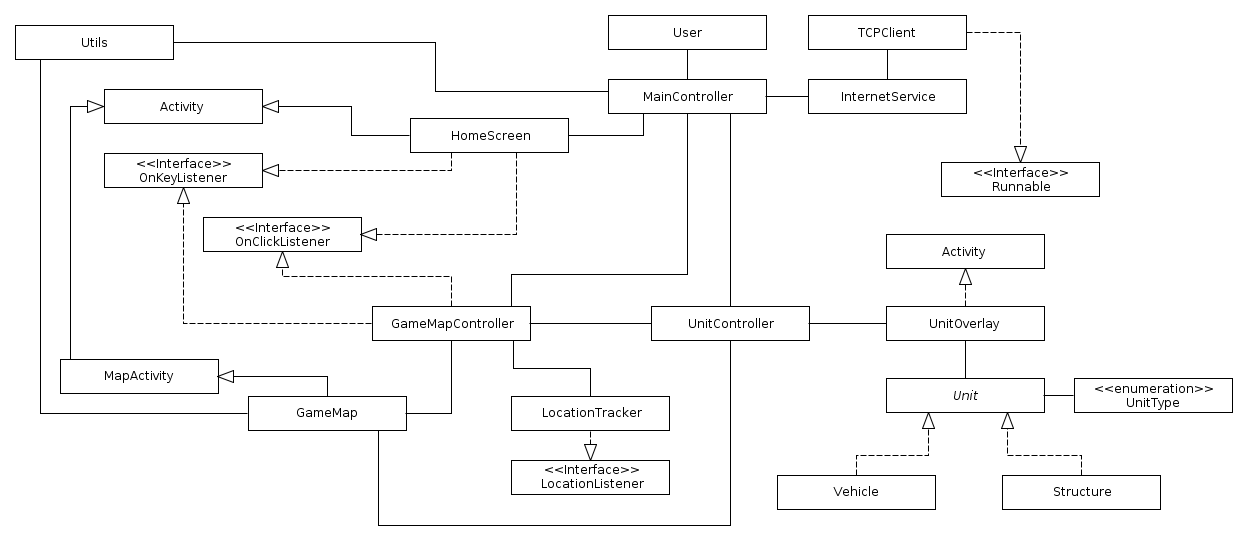
\includegraphics[height=0.29\textheight, angle=-90]{Images/diagrams/class.png}
\end{figure}



\chapter{Server Testing - Message Generator}\label{server_testing}

\begin{lstlisting}
#!/usr/bin/env python
import socket
import sys
import time
import re
import json


HOST = 'localhost'
PORT = 4565

sess = None
userID = None

try:
  sock = socket.socket(socket.AF_INET, socket.SOCK_STREAM)
  sock.connect((HOST, PORT))
except socket.error, msg:
  sys.stderr.write("[ERROR] %s\n" % msg[1])
  sys.exit(1)


while True:
  n = raw_input("> ")

  msgDic = dict()

  if n == "exit":
    break  # stops the loop
  else:
    match = re.findall("[^\s]+", n, re.M|re.I)
    if match:
      if match[0] == 'login':
        msgDic['action'] = "user.login"
        msgDic['user'] = match[1]
        msgDic['pass'] = match[2]
      elif match[0] == 'register':
        msgDic['action'] = "user.register"
        msgDic['user'] = match[1]
        msgDic['pass'] = match[2]
        msgDic['email'] = match[3]
      elif match[0] == 'location':
        msgDic['action'] = "user.location"

        if len(match) == 3:
          msgDic['lat'] = match[1]
          msgDic['lon'] = match[2]
        else:
          msgDic['lat'] = '52.35184333541474'
          msgDic['lon'] = '-1.966477632522583'
      elif match[0] == 'unit':
        msgDic['action'] = "unit.create"
        msgDic['type'] = match[1]
        msgDic['lat'] = match[2]
        msgDic['lon'] = match[3]
      elif match[0] == 'move':
        msgDic['action'] = "unit.move"
        msgDic['id'] = match[1]
        msgDic['lat'] = match[2]
        msgDic['lon'] = match[3]
      else:
        continue
      
      if sess:
        msgDic['sess'] = sess
      if userID:
        msgDic['userID'] = userID

      msg = json.dumps(msgDic)
      print '\x1b[38;5;15m' + "S " + msg + '\033[0m'
      sock.send(msg)


    else:
      continue


  rec = sock.recv(2048)
  try:
    data = json.loads(rec)

    #check for session data
    if data['action'] == 'user.login' and data['status'] == 1:
      sess = data['sess']
      #sess = 'cat'
      userID = data['userID']

    if data['status'] == 1:
      print '\x1b[38;5;46m' + "R " + rec + '\033[0m'
    else:
      print '\x1b[38;5;160m' + "R " + rec + '\033[0m'
  except ValueError:
    print rec


sock.close()

sys.exit(0)

\end{lstlisting}